% !TEX root = USEGUIDE.tex
\pagenumbering{arabic}


\part{Introduction}

    \begin{figure}[H]
    \centering
    \centerline{
\includegraphics[scale=0.2]{LOGO_CLASS.png}}
    \caption{CLASS logo}
    \label{fig:CLASSLogo}
    \end{figure}

    \vspace{2cm}

The code CLASS (\textbf{C}ore \textbf{L}ibrary for \textbf{A}dvanced \textbf{S}cenario \textbf{S}imulation) is a dynamic fuel cycle simulation tool developed by CNRS/IN2P3 (Centre National de la Recherche Scientifique / Institut National de Physique Nucléaire et de Physique des Particules) in collaboration with IRSN (Institut de Radioprotection et de Suret\'e Nucl\'eaire). The aim of the tool CLASS is to model an evolving electro-nuclear fleet. The main output is the evolution of isotopes in all facilities of a nuclear fleet. The reactor physics is located in the treatment of the fuel fabrication and its depletion in reactor. The code CLASS aims to be a useful tool for scenarios studies. CLASS main asset is its ability to implement any kind of reactor, either the system is innovative or standard. Indeed, the opportunity is given to each user to \textbf{build his own reactor model}.

\part{First Steps}
\chapter{Package Content}
The CLASS package contains the followings :
\begin{itemize}
\item   \textbf{data/} : folder containing nuclei properties
\subitem \textbf{FPyield\_Fast\_JEFF3.1.dat }     : file containing fission yield for fast reactors
\subitem \textbf{FPyield\_Thermal\_JEFF3.1.dat}   : file containing fission yield for thermal reactors
\subitem \textbf{Mass.dat }                     : file containing molar masses
\subitem \textbf{SpontaneousFPyield.dat }       : file containing spontaneous fission yields
\subitem \textbf{chart.JEF3T}                   : file containing decay constants and branching ratios
\subitem \textbf{HeatTox.dat}                   : file containing conversion data for heat and radiotoxicity calculation

 \item \textbf{DATA\_BASES/}  : this folder contains decay data base and reactor data bases
 \subitem \textbf{DECAY/}     : decay data base
 \subitem \textbf{FBR-Na/}    : Models related to Fast reactor
 \subitem \textbf{PWR/}       : Models related to Pressurised Water Reactor
 \subitem \textbf{REP\_HFC/}   : Models related to low moderated Pressurised Water Reactor 
 \subitem \textbf{ADS/}       : Models related to Accelerator Driven System
 
 \item \textbf{documentation/} 
 \subitem \textbf{Manual/}    : folder containing this user guide an its .tex sources
 \subitem \textbf{Doxygen/}   : folder containing the builded doxygen and its generation configuration 

\item \textbf{example/} : folder containing simple examples of CLASS input and an example of CLASS ouput reader

\item \textbf{gui/} : folder containing sources of the graphical user interface for CLASS outputs
 
\item \textbf{lib/} : folder containing the CLASS library (once compiled)
\item \textbf{bin/} : folder containing the CLASSGui and the Google test binary (once compiled)

\item \textbf{source/} : folder containing CLASS sources
\subitem \textbf{include/}
\subitem \textbf{Model/} : folder that contain the sources related to the physics models (EquivalenceModel , XSModel and IrradiationModel)
\subitem \textbf{src/}
\subitem \textbf{External/} : folder that contain the sources related to external classes used by the code CLASS

\item \textbf{Utils/} : folder containing utility software related to reactor data base generation
\subitem \textbf{EQM/} : Example of software to generate equivalence model for building reactor fuel
\subitem \textbf{MURE2CLASS/} : Software to convert MURE (a fuel depletion code)  output to \hyperref[sec:EvolutionData]{EvolutionData} format
\subitem \textbf{XSM/} : Software to generate cross section predictor
\subitem \textbf{ROOT2DAT/} : Software to convert CLASS output into readable ASCII data file
\subitem \textbf{ROOT2ROOT/} : Software to convert multiple CLASS Output into one single ROOT file (used for sensitivity analysis)
 
\end{itemize}

\chapter{Install procedure}

\section{Requirement}

\begin{itemize}
\item User skills : Good knowledge of C++. Experience in depletion codes and neutron transport codes is required for building complex new reactor model.
\item OS : CLASS is known to work under Linux (64  bits) and MacOSX (64 bits). It  has never been tested on any Windows distribution.
\item C++ compiler :  we recommend to use a gnu compiler like gcc4.8 or above. For OSX, CLASS is working with native clang compiler.
\item For DARWIN (OSX) users : 
Make sure you have installed XCode and its command line tools (if not dowload and install from AppStore). If using clang compiler, there's no possibility to use openmp. 
\item Root (CERN) :  
ROOT~\cite{Brun_1997} is an analysis software developped by CERN. CLASS version 5 uses some ROOT version 6 features to run. CLASS uses Root to store output data. The graphical user interface CLASSGui is also based on Root. Some algorithms uses the TMVA module of Root. 
\end{itemize}

\section{Installation}

\subsection{Get the source from archive}

Download the source of CLASS at the following adress : \href{https://gitlab.in2p3.fr/sens/CLASS/tree/master}{gitlab link}. The archive is available at the location showed on figure\ref{fig:CLASSArchive}.

    \begin{figure}[H]
    \centering
    \centerline{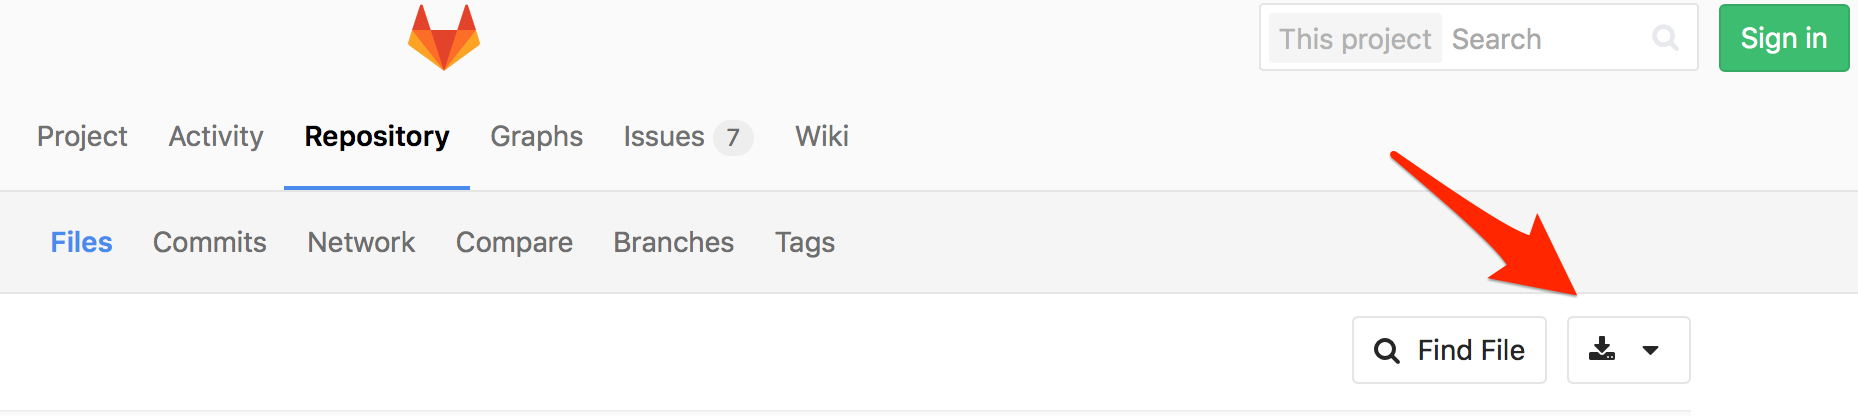
\includegraphics[width=0.99\textwidth]{GitlabDownload.png}}
    \caption{Archive for source of CLASS}
    \label{fig:CLASSArchive}
    \end{figure}

\subsection{from git public repository}

It is also possible to clone the git repository with the following commands : 

\begin{center}
\begin{minipage}{\textwidth}
\begin{lstlisting}[style=terminal]
cd YourProgDirectory
git clone https://gitlab.in2p3.fr/sens/CLASS.git
\end{lstlisting}
\end{minipage}
\end{center}

\subsection{CLASS Compilation}

Run the following command for a complete install with associated google tests (remove option -gtest if you don't want the tests to run) : 

\begin{center}
\begin{minipage}{\textwidth}
\begin{lstlisting}[style=terminal]
./install.sh -build -gtest
\end{lstlisting}
\end{minipage}
\end{center}

\subsection{Environment variables definition}

At this step, you'll need to define environnement variables in your shell environnment configuration file (.bashrc, .cshrc, .zshrc, etc...). 

\begin{itemize}
\item CLASS\_PATH : "CLASSDirectoryNameOfYourChoice"

\item CLASS\_lib : "\$CLASS\_PATH/lib"
\item PATH : "\$\{PATH\}\:\$CLASS\_PATH/bin"

\item CLASS\_include : "\$CLASS\_PATH/source/include"
\item CLASS\_external : "\$CLASS\_PATH/source/external"
\item CLASS\_Equivalence : "\$CLASS\_PATH/source/Model/Equivalence"
\item CLASS\_Irradiation : "\$CLASS\_PATH/source/Model/Irradiation"
\item CLASS\_XS : "\$CLASS\_PATH/source/Model/XS"

\item CLASS\_CFLAG : "-I\$CLASS\_include -I\$CLASS\_external -I\$CLASS\_Equivalence -I\$CLASS\_Irradiation -I\$CLASS\_XS -L\$CLASS\_lib -lCLASSpkg `root-config --cflags` `root-config --libs`"

\item LD\_LIBRARY\_PATH : "\$\{LD\_LIBRARY\_PATH\}\:\$\{CLASS\_lib\}"
\item DYLD\_LIBRARY\_PATH : "\$\{DYLD\_LIBRARY\_PATH\}\:\$\{CLASS\_lib\}"
\end{itemize}

\chapter{CLASS Execution}
CLASS is a set of C++ libraries, there is no CLASS binary file. A CLASS executable has to be build by user using objects and methods defined in the CLASS package.

After CLASS compilation, you can run the set of example defined in the directory example. 


The compilation line for generating your executable from a .cxx file is the following :
(You can find CLASS input examples in \$CLASS\_PATH/example/)

\begin{center}
\begin{minipage}{\textwidth}
\begin{lstlisting}[style=terminal]
g++ -o CLASS_exec YourScenario.cxx -I $CLASS_include -L $CLASS_lib -lCLASSpkg `root-config --cflags` `root-config --libs` -fopenmp -lgomp -Wunused-result -lTMVA
\end{lstlisting}
\end{minipage}
\end{center}
Then type 
\begin{center}
\begin{minipage}{\textwidth}
\begin{lstlisting}[style=terminal]
./CLASS_exec
\end{lstlisting}
\end{minipage}
\end{center}

The following should show in your terminal :

    \begin{figure}[H]
    \centering
    \centerline{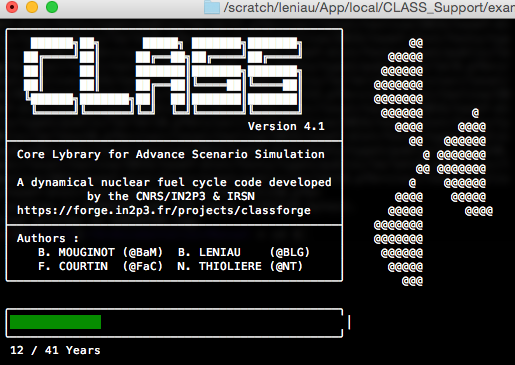
\includegraphics[scale=0.9]{CLASS_Run.png}}
    \caption{CLASS running in a shell}
    \label{fig:CLASSRUN}
    \end{figure}




\chapter{News, forum, troubleshooting, doxygen ...}
CLASS has a \href{https://forge.in2p3.fr/projects/classforge}{forge}\footnote{https://forge.in2p3.fr/projects/classforge} hosted by the IN2P3  where you can find :

\begin{itemize}
\item \href{https://forge.in2p3.fr/projects/classforge/boards}{A forum}\footnote{https://forge.in2p3.fr/projects/classforge/boards} where you are invited to post your trouble about CLASS installation and usage. You may find the answer to your trouble on a already posted thread.
\item \href{https://forge.in2p3.fr/projects/classforge/embedded/doxygen/inherits.html}{A doxygen}\footnote{https://forge.in2p3.fr/projects/classforge/embedded/doxygen/inherits.html} where all the CLASS objects and methods are defined and explained. Note that the doxygen is also contained in \$CLASS\_PATH/documentation/doxygen/CLASSDoxygen.html
\item \href{https://forge.in2p3.fr/projects/classforge/news}{News}\footnote{https://forge.in2p3.fr/projects/classforge/news} : All the news related to CLASS
\end{itemize}
A \href{classuser-l@ccpntc02.in2p3.fr}{Mailing List}\footnote{classuser-l@ccpntc02.in2p3.fr} also exist in order to be warned of all the change inside CLASS and to allow user to exchange directly on the code. One can join the mailing list through the following  \href{http://listserv.in2p3.fr/cgi-bin/wa?SUBED1=classuser-l&A=1}{link}\footnote{http://listserv.in2p3.fr/cgi-bin/wa?SUBED1=classuser-l\&A=1}.



